\chapter{Desenvolvimento}
\label{cap:desenv}

A partir de agora, será descrito o desenvolvimento do trabalho propriamente dito. Espera-se que as revisões, até o momento, tenham sido suficientes para a compreensão total do mesmo.

Para a execução dos treinos, fez-se necessário revisar a formatação do PTB, e dos dois \textit{treebanks} a serem convertidos. O procedimento de conversão, no geral, é basicamente o mesmo. Em primeiro lugar, a estrutura da sentença já classificada é refeita de forma lógica, remontando-a numa estrutura de dados em formato de árvore. Neste processo, as traduções das \textit{POS tags} são feitas. No segundo momento, caso a árvore recém traduzida possua alguma \textit{tag} que exija uma verificação mais aprofundada, esse tratamento é realizado. Esta segunda etapa ocorre de acordo com a necessidade, não sendo obrigatória para todas as sentenças. Por fim, a estrutura de dados é convertida para texto, respeitando o \textit{bracketing} do PTB.

O leitor pode se perguntar sobre a necessidade da segunda etapa, se um dos objetivos deste trabalho é, justamente, que não seja necessário muito desenvolvimento. Infelizmente, sem esse tratamento mais cuidadoso, o \textit{parser} é incapaz de ser treinado, ou de classificar sentenças. 


\section{Treinando o Stanford Parser sobre CINTIL}
\label{treinando_sp_cintil}

O pacote obtido, com o CINTIL, contém um guia de instruções \cite{narrativeDescriptionCintil}, e o \textit{treebank} propriamente dito em formato XML\footnote{\url{https://www.w3.org/XML/}}. Para melhor uso, e melhor aplicação das árvores tanto para treino como para testes, fez-se necessária a separação deste arquivo em arquivos menores. Foi construído um \textit{script} na linguagem Python para fazer tal separação, gerando dois tipos de arquivo: as sentenças originais (\textquote{\textit{raw}}), e suas árvores (\textquote{\textit{tree}}).

Este único trabalho não é suficiente. 
% As \textit{POS tags} do CINTIL estão em Português, e para o uso delas pelo SP sem uso de pacotes, seria necessário traduzi-las para o Inglês. 
O CINTIL tem o próprio \textit{tagset} e, para que o mesmo possa ser utilizado no SP sem o uso de pacotes, faz-se necessário transduzí-las para o padrão PTB, que é aceito pelo \textit{parser}.
Fizemos então a conversão dessas \textit{tags}, de acordo com a Tabela \ref{tab:tab_cintil}. Note que \textit{tags} que possuem tradução direta (exemplo: Adjetivo, A e JJ) não foram especificadas nas observações.

Outra dificuldade é que, como supracitado, o \textit{tagset} informado no site oficial do CINTIL está defasado com relação ao \textit{treebank} real. O \textit{tagset} mais confiável, a respeito, é o \textquote{CINTIL TreeBank Handbook} \cite{cintil_handbook}. Foram usadas as \textit{tags} listadas nele, e as que ocorrem no \textit{treebank} concreto e que não foram previstas no \textit{Handbook} (Por exemplo, P’, C’ etc).

\begin{center}
\begin{longtable}{|p{0.15\linewidth}|p{0.2\linewidth}|p{0.15\linewidth}|p{0.15\linewidth}|p{0.3\linewidth}|}
\caption{Tabela de conversão: CINTIL para PTB}\\
\hline
\textbf{Tag Original (Português)} & \textbf{Nome da Tag} & \textbf{Tag Convertida} & \textbf{Ocorrências} & \textbf{Observações}\\
\hline
\endfirsthead
\multicolumn{5}{c}%
{\tablename\ \thetable\ -- \textit{Continuação da página anterior}} \\
\hline
\textbf{Tag Original (Português)} & \textbf{Nome da Tag} & \textbf{Tag Convertida} & \textbf{Ocorrências} & \textbf{Observações} \\
\hline
\endhead
\hline \multicolumn{5}{r}{\textit{Continua na próxima página}} \\
\endfoot
\hline
\endlastfoot
    A & Adjetivo & JJ & 5527 & \\
    A' & Sintagma Adjetival & ADJP & 114 & \\
    ADV & Advérbios & RB & 5510 & \\
    ADV' & Sintagma Adverbial & ADVP & 912 & \\
    ADVP & Sintagma Adverbial & ADVP & 428 & \\
    AP & Sintagma Adjetival & ADJP & 1456 & \\
    ART & Artigo & DT & 15583 & \\
    ART' & Artigo & NP & 1 & Equivaleria ao constituinte interemediário do \textit{Determiner Phrase} (DP) \citeonline{mioto2013novo}. Porém, PTB não prevê esse tipo de estrutura. O sintagma mais indicado para receber determinantes (artigos) foi, portanto, NP\\
    C & Complementador & CC & 275 & Será explicado na sessão \ref{subsec-cintil-c}\\
    C' & Sintagma Complemental & \_CP\_ & 2 & Será explicado na sessão \ref{subsec-cintil-c}\\
    CARD & Cardinais & CD & 2028 & Números cardinais\\
    CARD' & Sintagmas Cardinais & NP & 504 & PTB prevê que conjuntos de números são marcados como NP\\
    CL & Clíticos & PRP & 717 & No CINTIL, ocorre apenas como pronome. De acordo com \citeonline{cintil_handbook}, \textquote{\textit{A clitic pronoun has category CL. It is the head of an NP.}}\\
    CONJ & Conjunções & CC & 2460 & Será explicado na sessão \ref{subsec-cintil-conj}\\
    CONJ' & Sintagma Conjuntivo & \_CONJP\_ & 92 & Será explicado na sessão \ref{subsec-cintil-conj}\\
    CONJP & Sintagma Conjuntivo & CONJP & 609 & Será explicado na sessão \ref{subsec-cintil-conj}\\
    CP & Sintagma Complemental & SBAR & 1434 & Será explicado na sessão \ref{subsec-cintil-c}\\
    D & Artigo & DT & 29 & \\
    D1 & Quantificadores & DT & 1 & Não ocorre no Handbook, só no site. Único caso em que essa \textit{tag} aparece, D1 se comporta como Artigo\\
    D2 & Quantificadores & JJ & 1 & Não ocorre no Handbook, só no site. Único caso em que essa \textit{tag} aparece, D2 se comporta como Adjetivo\\
    DEM & Demonstrativos & DT & 1013 & Para o PTB, \textit{this}, \textit{that}, \textit{these}, \textit{those} são, também, determinantes. Logo, DT\\
    ITJ & Interjeições & UH & 4 & \\
    ITJ' & Sintagma de Interjeição & INTJ & 4 & Pelo manual de \textit{bracketing} do PTB, \textquote{\textit{INTJ | Interjection. Corresponds approximately to the part-of-speech tag UH (see the POS guidelines [Santorini 1990]).}}\footnote{\textquote{Interjeição. Corresponde aprocimadamente à etiqueta morfossintática UH (veja as diretrizes [\citeonline{posPTBguidelines}]}. Tradução própria.}\\
    N & Substantivo & NNS & 32989 & \\
    N' & Sintagmas Nominais & NP & 18043 & \\
    NP & Sintagmas Nominais & NP & 32258 & \\
    ORD & Ordinais & CD & 378 & PTB não prevê o uso de ordinais. Ou melhor: eles costumam ser postos em locuções nominais.\\% Não é uma boa transdução\\
    P & Preposição & IN & 13920 & \\
    P' & Sintagmas Preposicionais & PP & 337 & Não ocorre no Handbook\\
    PERCENT & simbolo percentual & NN & 164 & Nota 1: pode ser pronome + substantivo também (\textquote{por cento}). Nota 2: PTB considera o \% como NN (\textit{single noum})\\
    PERCENT' & Sintagma percentual & NP & 80 & PTB considera como NP\\
    PERCENTP & Sintagma percentual & NP & 36 & \\
    PNT & Pontuação & ? & 14748 & Explicado na sessão \ref{subsec:cintil-pnt}\\
    POSS & Possessivos & PP\$ & 620 & \\
    POSS' & Possessivos & NP & 10 & Não existe um sintagma pronominal no PTB. Mantivemos como NP\\
    PP & Sintagmas Preposicionais & PP & 15382 & \\
    PRS & Pronomes Pessoais & PRP & 395 & \\
    QNT & Quantificadores & PRP & 889 & De acordo com (\citeonline[p~55]{Castilho2010gramatica}), \textquote{Os pronomes abrigam as seguintes subclasses [...]: pessoais, demonstrativos, possessivos e quantificadores [...]}\\
    QNT' & Sintagma de Quantificadores & NP & 19 & Como supracitado, se refere ao sintagma que abriga quantificadores (pronomes)\\
    REL & Relativos & PRP & 861 & Pronomes relativos\\
    S & Sentença & S & 24393 & \\
    V & Verbos  & VB & 13281 & \\
    V' & Sintagma Verbal & VP & 2745 &  \\
    VP & Sintagma Verbal & VP & 15284 & 
\label{tab:tab_cintil}
\end{longtable}
\end{center}

Como veremos também ao trabalharmos com o Bosque, nem todo caso pode ser feito com uma simples tradução direta CINTIL $\rightarrow$ PTB. Em alguns momentos, tivemos que avaliar, para cada caso, como traduzir a \textit{tag} de maneira correta. Estes casos serão descritos abaixo
% ------------------------------------------------------------------------------------------------
\subsection{Problemas com CONJ (Conjunção)}
\label{subsec-cintil-conj}
Conjunções são estruturas (palavras, no geral) que fazem parte da categoria semântica da Conectividade. Descrita por \citeonline[p~133]{Castilho2010gramatica},
\begin{displayquote}
    \textquote{Outra categoria semântica é a conectividade, gramaticalizada como preposições e conjunções. Essas classes ligam palavras e sentenças, com a diferença de que as preposições, como classe igualmente predicadora, atribui ao seu escopo traços de lugar, tempo, entre outros, propriedade não exercida pelas conjunções.}
\end{displayquote}
O mesmo autor descreve que sentenças podem ser ligadas por conjunções e que, ao fazê-lo, estamos criando uma relação conjuncional entre ambas. \citeonline[p~338]{Castilho2010gramatica}:
\begin{displayquote}
    \textquote{Essa relação compreende a [\ldots] coordenação, [\ldots] formada por sentenças independentes umas de outras, ou de [\ldots] subordinação, [\ldots] formada por sentenças encaixadas umas em outras, tanto quanto [\ldots] formada por uma sentença adjunta à outra.}
\end{displayquote}
A Tabela 
% \ref{tab:tab_conj_separadas_cintil} e 
\ref{tab:tab_conj_concat_cintil} mostra palavras e expressões utilizadas pelo CINTIL como conjunções.
% \begin{center}
% \begin{table}[!ht]
    \centering
    \begin{tabular}{|l|l|l|l|}
        \hline
        a & e & nem & se\\
        ainda & em & não & sem\\
        assim & em\_ & o & sempre\\
        até & embora & ou & só\\
        bem & enquanto & para & também\\
        caso & já & porque & tanto\\
        como & mais & quando & uma\\
        dado & mas & quanto & vez\\
        de\_ & medida & que & \\
        desde & mesmo & quer & \\
        \hline
    \end{tabular}
    \caption{Palavras únicas usadas como conjunções pelo cintil. Note que palavras com underline (\_) são concatenadas a outras (no geral, indica uma preposição)}
    \label{tab:tab_conj_separadas_cintil}
\end{table}
% \end{center}
\begin{center}
\begin{table}[!ht]
    \centering
    \begin{tabular}{|l|l|}
        \hline
        ainda que&mas\\
        até que&mesmo que\\
        dado que&ou\\
        de\_ o que&para que\\
        desde que&sem que\\
        e&tanto mais que\\
        em\_ a medida em que&uma vez que\\
        já que&\\
        \hline
    \end{tabular}
    \caption[Expressões usadas como conjunções pelo CINTIL]{Expressões (conjuntos de palavras, ou palavras únicas) usadas como conjunções pelo CINTIL. Note que as preposições com \textit{underline} se concatenam ao artigo posterior (de\_ + o = do)}
    \label{tab:tab_conj_concat_cintil}
\end{table}
\end{center}

O \textit{Penn Treebank} e o CINTIL lidam com conjunções de maneiras distintas. O PTB, em seu manual de anotação \cite[p~117]{bracketing_ptb}, dedica a seção 7.5 para descrever tal fenômeno. Lá podemos ver que, para conjunções coordenadas, temos três casos: palavra simples (\textit{and}, \textit{but}, \textit{or}, \ldots), multi palavra (\textit{as well as}, \textit{not to mention}, \textit{rather than}, \ldots), e conjunções descontínuas (\textit{not only\ldots but}, \textit{not\ldots but instead}, \ldots). Palavras simples não precisam de marcação, a conjunção fica sem rótulo, como na Figura \ref{fig:ptb_conj_exe_1}. Conjunções com várias palavras tem o sintagma de conjunção marcado como CONJP, e as conjunções são postas em estrutura plana, mostrado na Figura \ref{fig:ptb_conj_exe_2}. Por fim, conjunções descontínuas tem apenas a parte com múltiplas palavras marcada por CONJP. A palavra isolada permanece isolada e sem marcação, como na Figura \ref{fig:ptb_conj_exe_3}. O manual possui a descrição de mais casos, envolvendo Conjunções Coordenadas e \textit{times}\footnote{\textit{Vezes}, no sentido de multiplicação. Exemplo, \textit{three times}, ou \textit{three times five}}, porém não nos alongaremos no assunto, por não possuírem as \textit{tags} CONJ ou CONJP.
\begin{center}
\begin{figure}[!h]
    \centering
    % \includegraphics{}
    \begin{minipage}{10cm}
        \begin{tabbing}
            \=(NP \=(NP a hammer)\+\\
            \>\textbf{and}\\
            \>(NP a nail))\\
        \end{tabbing}
    \end{minipage}
    \caption[Exemplo de conjunção coordenada (\textit{single-word})]{Exemplo de conjunção coordenada com uma palavra (\textit{single-word}). Adaptado de \citeonline[p~130]{bracketing_ptb}}
    \label{fig:ptb_conj_exe_1}
\end{figure}
\end{center}
\begin{center}
\begin{figure}[!h]
    \centering
    % \includegraphics{}
    \begin{minipage}{10cm}
        \begin{tabbing}
            \=(S (\=NP-SBJ That)\+\\
                \>(VP \=builds\+\\
                    \>(NP (NP confidence)\\
                    \>,\\
                    \>(NP self sufficiency)\\
                    \>,\\
                    \>\textbf{(CONJP not to mention)}\\
                    \>(NP critical regulatory net worth)))\-\\
                \>.)
        \end{tabbing}
    \end{minipage}
    \caption[Exemplo de conjunção coordenada \textit{multi-word}]{Exemplo de conjunção coordenada com muitas palavras (\textit{multi-word}). Adaptado de \citeonline[p~131]{bracketing_ptb}}
    \label{fig:ptb_conj_exe_2}
\end{figure}
\end{center}
\begin{center}
\begin{figure}[!h]
    \centering
    % \includegraphics{}
    \begin{minipage}{10cm}
        \begin{tabbing}
            \=(S (\=NP-SBJ The proposal)\+\\
                \>(VP \=represents\+\\
                    \>(NP \=\textbf{(CONJP not alone)}\+\\
                    \>(NP his own district)\\
                    \>\textbf{but}\\
                    \>(NP (NP all the people)\\
                    \>(PP \=of\\
                        \>(NP our country))))))\\
        \end{tabbing}
    \end{minipage}
    \caption[Exemplo de conjunção discontínua]{Exemplo de conjunção discontínua (\textit{discontinuous conjunction}). Adaptado de \citeonline[p~131]{bracketing_ptb}}
    \label{fig:ptb_conj_exe_3}
\end{figure}
\end{center}

O CINTIL, por outro lado, não é tão descritivo. É dito em \cite[p~20]{cintil_handbook}:
\textquote{\textit{Coordination of two constituents A and B by means of a coordinative conjunction Conj (either a lexical item, such as \textit{e}, or a comma) are a cascade of adjunctions [A [Conj [ B ]]].}}
\footnote{\textquote{Coordenação de dois constituintes A e B no sentido de uma conjunção coordenada Conj (tanto um item lexical, como \textit{e}, ou uma vírgula) são uma cascata de adjunções [A [Conj [B]]].}}
% Ele prevê as tags CONJ, CONJP e CONJ’.
Pela observação do \textit{treebank}, vemos CONJP se refere a toda a nova sentença em conjunção com a sentença inicial. CONJ’ se refere ao núcleo da conjunção (aos moldes da estrutura CP, que pode ser vista em \cite[p~63]{mioto2013novo}). Por fim, CONJ é a \textit{POS tag} referente a conjunções.

CINTIL abarca toda a nova sentença da conjunção, como demonstrado na Figura \ref{fig:cintil_conj_exe_1}. Como visto anteriormente, o mesmo não ocorre no PTB. Conjunções normalmente não são marcadas e, se forem, receberam a marca CONJP para o núcleo.
% \footnote{Também ocorre a conjunção marcada por SBAR, mas não há necessidade de explorarmos. Para o leitor curioso, recomendamos a leitura de \citeonline[sec~1.2.3]{bracketing_ptb}}1.
\begin{center}
\begin{figure}[!h]
    \centering
    % \includegraphics{}
    \begin{minipage}{.8\textwidth}
        \begin{tabbing}
            \=(S  \=\+\\
            \>    (S  \=\+\\
            \>        (NP  \=\+\\
            \>            (ART o) (N Manuel)\-\\
            \>        )\\ 
            \>        (VP  \=\+\\
            \>            (V é\=) \\
            \>            (AP \+\\
            \>               (A maior) \\
            \>                (CON\=JP \+\\
            \>                    (CON\=J' \+\\
            \>                        (CONJ de\_) (CONJ o) (CONJ que)\-\\
            \>                    ) \\
            \>                    (NP \=\+\\
            \>                        (ART A) (N Maria)\-\\
            \>                    ))))) \-\-\-\-\\
            \>    (PNT .)\-\\
            \>)
        \end{tabbing}
    \end{minipage}
    \caption[Exemplo de conjunção no CINTIL]{Sentença aTSTS-001/36, \textquote{o Manuel é maior do que A Maria}. Exemplo de conjunção no CINTIL (Adaptado)}
    \label{fig:cintil_conj_exe_1}
\end{figure}
\end{center}

Com isto em mente, fez-se necessário reescrever a disposição das \textit{tags}, para que: CONJP se referisse apenas aos núcleos conjuntivos, CONJ’ fosse removida e, no contexto em que CONJ aparece dentro de \textit{tags} CONJP, remover suas marcações, sem removê-las noutros momentos. Um exemplo pode ser visto na Figura \ref{fig:cintil_conj_exe_2}.
\begin{center}
\begin{figure}[!ht]
    \centering
    % \includegraphics{}
    \begin{minipage}{10cm}
        \begin{tabbing}
            \=(S\=\+\\ 
            \>  (S\=\+\\ 
            \>    (NP\=\+\\ 
            \>      (DT o)\\
            \>      (NNS Manuel)\=\-\-\\
            \>    )\\
            \>    (VP\=\+\\ 
            \>      (VB é)\\
            \>      (ADJP\=\+\\ 
            \>        (JJ maior)\\
            \>        (CONJP de\_ o que)\\
            \>        (NP\=\+\\ 
            \>          (DT A)\\
            \>          (NNS Maria)\-\\
            \>        )\-\\
            \>      )\-\\
            \>    )\-\\
            \>  )\\
            \>  .)\\
        \end{tabbing}
    \end{minipage}
    \caption[Sentença aTSTS-001/36, modificada para se adaptar ao PTB]{Sentença aTSTS-001/36, \textquote{o Manuel é maior do que A Maria.}, modificada pelo algoritmo desenvolvido para se adaptar ao PTB}
    \label{fig:cintil_conj_exe_2}
\end{figure}
\end{center}

\subsection{Problemas com C (Complementizador)}
\label{subsec-cintil-c}

Semelhante à CONJ em diversos aspectos, as \textit{tags} C, C’ e CP permitem a conjunção entre sentenças, tornando uma segunda sentença objeto de uma primeira. O tratamento feito com elas foi muito semelhante ao dado para a \textit{tags} CONJ, com um diferencial: CONJ’ ocorre sem necessariamente ter a \textit{tags} CONJP como pai (12 casos), o que nunca ocorre com a família CP. 

\subsection{Problemas com PNT (Pontuação)}
\label{subsec:cintil-pnt}

Foi observado, também, que CINTIL e PTB lidam com pontuações de formas distintas. CINTIL usa a \textit{tags} PNT para classificar estes símbolos. PTB prevê uma \textit{tags} SYM, para símbolos. Além disso, vemos em \cite[p~52]{buildingPTB} que os símbolos costumam ser representados sem etiquetas, como exemplificado na Figura \ref{fig:ptb_comma_parenthe}. Em \cite[p~52]{bracketing_ptb}, fica bastante claro: fora \textit{bracketing} (parênteses, colchetes, chaves), os símbolos não recebem nenhuma \textit{POS}. Quando recebe, como no caso de símbolos funcionando como palavras, ou símbolos matemáticos, são \textit{tags} referentes ao sintagma. Um detalhe importante é como PTB lida com aspas e apóstrofos (\textit{quote}, e \textit{single-quote}). As aspas são removidas, e substituídas por dois apóstrofos ou duas crases (melhor visualizado na Figura \ref{fig:ptb-quote}).

\begin{center}
    \begin{figure}[!ht]
    \centering
    % \includegraphics{}
    \begin{minipage}{10cm}
        \begin{tabbing}
            \=(   (S-1 \=\+\\ 
            \>    (PP-TMP \=For\+\\
            \>		(NP \=(NP the rest)\+\\
            \>			(PP \=of\+\\
            \>				\=(NP 1989))))\-\-\-\-\\
        	\>  (PRN \=,\+\\
            \>		(S \=(NP-SBJ Mr. Hagen) \+\\
            \>	        (VP \=said\+\\
            \>		        (SBAR \=0\+\\
            \>				    (S *T*-1))))\-\-\-\\
            \>		,)\-\\
            \>	(NP-SBJ \=(NP Conrail 's)\+\\
            \>		traffic and revenue)\-\\
            \>	''\\
            \>	(VP \=will\+\\
            \>		(VP \=reflect\+\\
            \>			(NP the sluggish economy)))\-\\
            \>	.))
        \end{tabbing}
    \end{minipage}
    \caption[Vírgulas marcando S entre parênteses]{Vírgulas marcando S entre parênteses (adaptado de \citeonline[p~52]{bracketing_ptb})}
    \label{fig:ptb_comma_parenthe}
\end{figure}
\end{center}

\begin{center}
    \begin{figure}[!h]
    \centering
    % \includegraphics{}
    \begin{minipage}{.8\textwidth}
        \begin{tabbing}
        \=((SINV \=\lq\lq\+\\
        \>    (S-TPC-1    \=(NP-SBJ We)\\
        \>                (VP \=have\+\\
        \>		            (NP \=(NP no useful information)\+\\
        \>			            (PP \=on\+\\
        \>			                (SBAR \=whether\+\\
        \>            				   (S \=(NP-SBJ users)\\
        \>            				      (VP \=are\+\\
        \>                					  (PP-\=PRD at\+\\
        \>                						  (NP risk)))))))))\\
        \>	\=, \\
        \>	\lq\lq\\
        \>  (VP \=said\+\\
        \>	    (S *T*-1))\-\\
        \>	(NP-\=SBJ (NP James A. Talcott)\+\\
        \>		(PP \=of\+\\
        \>		    (NP \=(NP Boston \lq s)\+\\
        \>			    Dana-Farber Cancer Institute)))\-\-\-\\
        \>	.))
        \end{tabbing}
    \end{minipage}
    \caption[Exemplo de uso de aspas no PTB]{Exemplo de uso de aspas no PTB (fragmento adaptado da sentença wsj\_0003)}
    \label{fig:ptb-quote}
\end{figure}
\end{center}

Fez-se necessário criar um \textit{script} que removesse as \textit{tags} PNT dos símbolos, do CINTIL, para reposicioná-los corretamente nas árvores, além de tratar \textit{quotes}.

% Porém, não podia ser tão simples, e não foi. 
Porém,
CINTIL não só identifica os PNT de forma diferentes, como também os POSICIONA de forma distinta, como podemos ver no comparativo da Figura \ref{fig:comp_PNT_ptb_cintil}. No exemplo, abordando ponto final, é definido em \cite[p~52]{bracketing_ptb}, 
\begin{quote}
    \textquote{\textit{In this corpus, each unit of text is enclosed in a top level of unlabeled brackets [\ldots]. Formerly, top-level punctuation [\ldots] could be attached to these top-level brackets. However, in this release, such punctuation should all be attached one level down (to the highest level of labeled brackets), so that there is only one top-level node within the unlabeled brackets.}}
    \footnote{\textquote{Neste corpus, cada unidade de texto é fechada no nível superior de parênteses não marcados [\ldots]. Anteriormente, pontuações de nível superior [\ldots] podiam ser anexadas àqueles parênteses de nível superior. Porém, nesta versão, tal pontuação deve toda ser anexada um nível abaixo (para o nível mais alto dos parênteses rotulados), então existe apenas um nó no topo dentro dos parênteses não rotulados}. Tradução própria.}
\end{quote}

E resume em \cite[p~57]{bracketing_ptb}: 
\textquote{\textit{Final punctuation as a rule is a child of the highest level of structure}}.
\footnote{\textquote{Ponto final é, por regra, um filho da estrutura de nível mais elevado}. Tradução própria.}
Já \cite[p~29]{cintil_handbook} define como \textquote{\textit{End of sentence markers are in the top most adjunction}}
\footnote{\textit{Marcadores de fim de sentença estão na adjunção mais ao topo}. Tradução própria.}.

\begin{center}
    \begin{figure}[!h]
    \centering
    % \includegraphics{}
    \begin{minipage}{0.5\textwidth}
        \centering
        \begin{forest}
            [ [S [NP-SBJ This]
            [VP is
            [NP-RPD [NP John]
            [\textbf{,}]
            [NP my brother]]]
            [\textbf{.}]]]
        \end{forest}
        \caption{\textquote{This is John, my brother.}}
    \end{minipage}%
    % \hfill
    \begin{minipage}{0.5\textwidth}
        \centering
        \begin{forest}
            [S [S [VP [VP [ADV Assim]] [ADV' [\textbf{PNT ,}] [ADV' [ADV tal] [ADV e] [ADV qual]]]]] [\textbf{PNT .}]]
        \end{forest}
        \caption{\textquote{Assim, tal e qual.}}
    \end{minipage}
    \caption[Comparativo entre posicionamento de sinais de pontuação entre o Penn Treebank e o CINTIL]{Comparativo entre posicionamento de sinais de pontuação entre o Penn Treebank e o CINTIL.}
    \label{fig:comp_PNT_ptb_cintil}
\end{figure}


\end{center}

Vírgulas também são bastante curiosas. Em \cite[p~52]{bracketing_ptb}: 
\begin{quote}
    \textquote{\textit{Paired punctuation marks are siblings of the constituents they surround. This is true even when the opening or closing member of the pair can be viewed as deleted. For instance, the commas that set off a subordinate clause or a relative clause from a main clause are siblings of the SBAR dominating the subordinate clause. [\ldots]}}
    \footnote{\textquote{Marcadores de pontuação pareados são irmãos do constituinte que eles rodeiam. Isto é verdade mesmo quando o membro inicial ou final do par pode ser visto como apagado. Por exemplo, as virgulas que definem uma cláusula subordinada ou clausula relativa de uma cláusula principal são irmãos do SBAR dominando a cláusula subordinada. [\ldots]}. Tradução própria.}
\end{quote}

Podemos ver esse fenômeno na Figura \ref{fig:ptb_comma_parenthe}. Já em \cite[p~30]{cintil_handbook}, 
\textquote{\textit{Commas separating left periphery constituents are right adjoined to theses constituents.}}
\footnote{\textquote{Vírgulas separando constituintes periféricos à esquerda são adjungidos à direita destes constituintes}, tradução própria}, exemplo na Figura \ref{fig:cintil_comma_left}.

\begin{center}
    \begin{figure}[!h]
    \centering
    % \includegraphics{}
    \begin{forest}
		[S [PNT '] [S [S [VP [V Falámos] [PP [PP [P de] [NP [N caça]]] [PP [\textbf{PNT ,}] [PP [PP [P de\_] [NP [ART os] [N sócios]]] [PP [CONJ e] [PP [P de] [NP [N' [N assuntos] [PP [P de] [NP [N homens]]]]]]]]]]]] [PNT .]]]
    \end{forest}
    \caption[Exemplo de comportamento da vírgula no CINTIL]{Exemplo de comportamento da vírgula no CINTIL. Vírgulas separando componentes periféricos à esquerda são anexados à direita do constituinte. Adaptado de \citeonline[p~30]{cintil_handbook}}
    \label{fig:cintil_comma_left}
\end{figure}
\end{center}

Para o leitor curioso, fica o Capítulo 3 de \cite{bracketing_ptb}, e 12 de \cite{cintil_handbook}, para o estudo dos demais sinais.

Antes de encerrarmos, existem casos no \textit{treebank} em que pontuações não são associadas à etiqueta PNT. Esses casos costumam ser pontos de abreviação, reticências, ou apóstrofos (\textit{single-quotes}) que antecedem nomes, e estão associados à etiqueta N. Para resolvê-los, primeiro mudamos suas etiquetas para PNT. Depois, continuamos com as operações previstas.

Fica claro, então, que é necessário \textit{reposicionar} os sinais antes de passar as árvores processadas para o SP. 
% parece um erro pequeno, mas 
Tal erro inviabiliza completamente qualquer tipo de teste, como podemos ver na mensagem de retorno exibida na Figura \ref{fig:cintil_training_error}. Num primeiro momento, a solução foi apenas remover tais elementos, o que viabilizou o treinamento e avaliação.

\begin{center}
    \begin{figure}[!h]
    \centering
    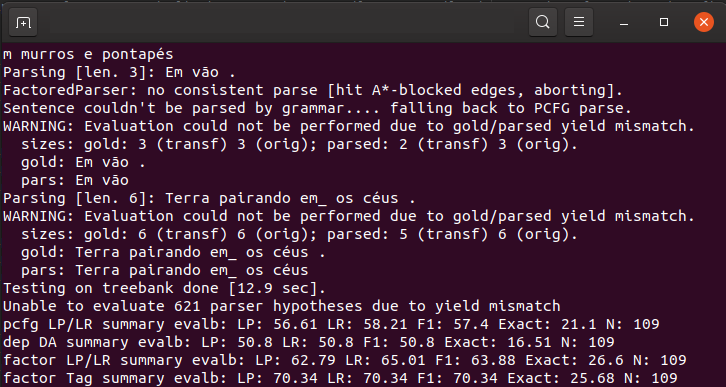
\includegraphics[width=100mm,scale=1.5]{imagens/cintil_training_error.png}
    \caption[Erro decorrente do mal posicionamento de pontuações na árvore do CINTIL]{Captura de tela de erro decorrente do mal posicionamento de pontuações na árvore do CINTIL, com relação ao formato PTB}
    \label{fig:cintil_training_error}
\end{figure}
\end{center}

% ------------------------------------------------------------------------------------------------
\subsection{Treinamento}
\label{subsec:treinamento_cintil}

Para fazer estas conversões, fizemos um \textit{script} disponível online\footnote{\url{ https://github.com/Fernandomn/treebank-transductor}}.

Com as \textit{tags} convertidas, foi feito o treinamento. O ato do treino é relativamente simples: deve-se, através do terminal do seu sistema, navegar até o diretório onde se encontra o \textit{stanford-parser.jar}, o arquivo que contém os \textit{parsers} do SP que utilizaremos. Estando no diretório correto, deve-se executar o comando \ref{lst:testeBasicoCintil}:

\begin{center}
\begin{lstlisting}[breaklines, caption={Execução de treinos do Stanford Parser para o CINTIL},label={lst:treinoBasicoCintil},language=Bash]
    java -cp ~/<diretorio de trabalho>/stanford-parser.jar -mx4g edu.stanford.nlp.parser.lexparser.LexicalizedParser -train ~/<diretorio do treebank>/tree-trad 1-1014 -saveToSerializedFile ~/<diretorio de armazenamento>/serialGrammarCINTIL -saveToTextFile ~/<diretorio de armazenamento>/textGrammarCINTIL
\end{lstlisting}
\end{center}

O código acima merece algumas explicações a parte, para quem não está familiarizado ao uso do SP pelo terminal.

\begin{center}
\begin{table}[h!]
    \centering
    \begin{tabular}{p{0.8\textwidth}}
        \begin{itemize}
            \item [-cp] \textit{ClassPath}. Indica o diretório onde se encontra a classe principal a ser executada
            \item [-mx4g] Quantidade de memória usada. No caso, 4 GB.
            \item [LexicalizedParser] \textit{Parser} utilizado, dentre os disponibilizados
            \item [-train] Treino. Logo em seguida, um diretório e a lista de arquivos a serem usados para treinar
            \item [-saveToSerializedFile] Salva o resultado do treino num arquivo binário, cujo diretório está indicado na sequência
            \item [-saveToTextFile] Salva o resultado do treino num arquivo de texto, cujo diretório está indicado na sequência
        \end{itemize}
    \end{tabular}
    \caption[Comandos para um treino simples do \textit{Stanford Parser}]{Comandos para um treino simples do \textit{Stanford Parser}, utilizando o terminal.}
    \label{tab:tab_treino_basico_cintil}
\end{table}
\end{center}

A Tabela \ref{tab:tab_treino_basico_cintil} mostra um fragmento das possibilidades de comandos a serem usados pela interface do terminal do SP. Note que usamos apenas 1014 arquivos nesta demonstração, que é um fração de 10\% dos arquivos / árvores do CINTIL disponíveis.

Para melhor verificação dos resultados, utilizamos o método de \textit{10-fold cross-validation}. Este método, como explicado por \citeonline{james2013introduction},
\begin{displayquote}
    \textquote{\textit{[\ldots] involves randomly dividing the set of observations into k groups, or folds, of approximately equal size. The first fold is treated as a validation set, and the method is fit on the remaining k -- 1 folds}}
    \footnote{\textquote{Esta abordagem envolve dividir aleatoriamente o conjunto de observações em k grupos, ou dobras, de tamanhos aproximadamente iguais. O primeiro grupo é tratado como conjunto de validação, e o método se encaixa nos k -- 1 grupos restantes}. Tradução própria.}.
\end{displayquote}

No nosso caso, dividimos nosso \textit{corpora} em 10 partes de 1014 sentenças. Fizemos o treinamento com 9 partes, e o teste com a parte restante, alternando as partes escolhidas. Os resultados serão apresentados na conclusão.

Na sequência, foi executado o treinamento com as partes restantes. De maneira análoga, no mesmo diretório, foi utilizado o comando \ref{lst:testeBasicoCintil}:

\begin{center}
\begin{lstlisting}[breaklines, caption={Execução de testes do Stanford Parser para o CINTIL},label={lst:testeBasicoCintil},language=Bash]
    java -cp stanford-parser.jar -mx4g edu.stanford.nlp.parser.lexparser.LexicalizedParser -loadFromSerializedFile /home/fernando/projeto-final-parsers/serialized-files/serialGrammarCINTIL1 input/sentencas_teste_cintil.txt

\end{lstlisting}
\end{center}

Que também merece explicações, na Tabela \ref{tab:tab_teste_basico_cintil}:
\begin{center}
\begin{table}[h!]
    \centering
    \begin{tabular}{p{0.8\textwidth}}
        \begin{itemize}
            \item [-cp] \textit{ClassPath}. Indica o diretório onde se encontra a classe principal a ser executada
            \item [-mx4g] Quantidade de memória usada. No caso, 4 GB.
            \item [LexicalizedParser] \textit{Parser} utilizado, dentre os disponibilizados
            \item [-writeOutputFiles ] Indica que os testes imprimirão arquivos de saída, a serem definidos
            \item [-outputFilesDirectory] Define o diretório onde os arquivos de saída serão escritos. 
            \item [-loadFromSerializedFile] Carrega a gramática serializada, gerada na execução de treinamento anterior
            \item [-testTreebank] Diretório onde se encontra o treebank a ser usado para teste. Os números no formato $a-b$ indicam o primeiro e o último arquivo, respectivamente. Números no formato $a-b,c-d$ indicam dois blocos de arquivos. Atente para não usar o mesmo bloco dos treinos, ou o parser passará por \textit{overfitting}, e terá resultados enviesados.
        \end{itemize}
    \end{tabular}
    \caption[Comandos para um teste simples do Stanford Parser]{Comandos para um teste simples do Stanford Parser, utilizando o terminal.}
    \label{tab:tab_teste_basico_cintil}
\end{table}
\end{center}

O resultado total dos testes resultou na extensa Tabela \ref{tab:cintil_result_full}, que pode ser vista nos apêndices. E os comentários dos resultados pode ser encontrado em \ref{resultados_cintil}.
\section{Treinando o Stanford Parser sobre Bosque}
\label{sec:treinando_sp_bosque}

Como já visto, o Bosque é disponibilizado em duas variantes, português brasileiro (BR) e português europeu (PT). Este trabalho foi feito considerando ambas, porém focando na variante brasileira.

Como descrito em \ref{subsec:florestasintatica}, cada nó das árvores do Bosque são muito ricos em informação sintática. Como descrito em \ref{subsec:PennTB}, o PTB é \textquote{pobre}, se posto em comparação. Coube, então, fazer a remoção das outras características, mantendo apenas as \textit{tags} de \textquote{forma}, que equivalem às \textit{POS tags}.

Uma dificuldade, é que o arquivo de entrada está no formato ISO-8859. Ao ser convertido para o formato de texto aceito pelo SP (UTF-8), vários caracteres especiais, como letras acentuadas, se perdem. Foi necessário fazer a conversão do arquivo fonte, antes de realizar as operações de transdução. O comando utilizado pode ser visto em \ref{lst:convertUTF8}:
\begin{center}
    \begin{lstlisting}[breaklines, caption={Conversão de arquivo ISO para UTF-8},label={lst:convertUTF8},language=Bash]
    $ iconv -f ISO-8859-1  Bosque_CF_8.0.PennTreebank.ptb -t UTF-8 -o Bosque_CF_PTB.txt
\end{lstlisting}

\end{center}
Assim como o CINTIL, parte importante do nosso trabalho foi transduzir as \textit{tags} do BOSQUE para o padrão PTB. Isso implicou em decisões que serão apresentadas na Tabela \ref{tab:tab_bosque}:

\begin{center}
    \begin{longtable}{|p{0.1\linewidth}|p{0.2\linewidth}|p{0.15\linewidth}|p{0.15\linewidth}|p{0.3\linewidth}|}
\caption{Tabela de conversão: BOSQUE para PTB}\\
\hline
\textbf{Tag Original (Português)} & \textbf{Nome da Tag} & \textbf{Tag Convertida} & \textbf{Ocorrências} & \textbf{Observações}\\
\hline
\endfirsthead
\multicolumn{5}{c}%
{\tablename\ \thetable\ -- \textit{Continuação da página anterior}} \\
\hline
\textbf{Tag Original (Português)} & \textbf{Nome da Tag} & \textbf{Tag Convertida} & \textbf{Ocorrências} & \textbf{Observações} \\
\hline
\endhead
\hline \multicolumn{5}{r}{\textit{Continua na próxima página}} \\
\endfoot
\hline
\endlastfoot
    acl & Forma Oracional averbais & ?? & 277 & Não possui conversão direta. Melhor explicado em \ref{subsec:tag_acl}\\
    adj & adjectivos & JJ & 3484 & \\
    adjp & Sintagma adjectivais & ADJP & 3367 & \\
    adv & advérbios & RB & 3052 & \\
    advp & Sintagma adverbiais & ADVP & 2288 & \\
    art & artigos & DT & 10742 & \\
    conj-c & conjunções coordenativa & CC & 1723 & Explicado na sessão \ref{subsec:cu}\\
    conj-s & conjunções subordinativa & IN & 798 & \\
    cu & sintagma evidenciador de relação de coordenação & \_CU\_ & 1744 & Será explicado na sessão \ref{subsec:cu}\\
    ec & prefixos & \_EC\_ & 80 & Será explicado na sessão \ref{subsec:sec_ec}\\
    fcl & Forma Oracional Finita & VP & 6040 & Sentenças onde os verbos não estão no infinitivo. Sintagma verbal\\
    icl & Forma Oracional não finita & VP & 1827 & Sentenças onde os veros estão conjugados. Sintagma Verbal\\
    intj & interjeições & UH & 22 & \\
    n & substantivos & NN & 15724 & \\
    n-adj & substantivos / adjectivos & NN & 174 & Pesquisa mostrou que são todas as ocorrências são substantivos\\
    np & Sintagma nominais & NP & 22981 & \\
    num & numeral & CD & 1625 & \\
    pp & Sintagma preposicionais & PP & 11576 & \\
    pron-det & pronomes determinativos & DT & 1580 & Pelo \citeonline{posPTBguidelines}, \textquote{\textit{This category includes [\ldots] the indefinite determiners \textit{another}, \textit{any}, \textit{some}, \textit{each}, \textit{either} [\ldots], \textit{neither} [\ldots], \textit{that}, \textit{these}, \textit{this} and \textit{those} [\ldots]}}. No português, também, por \citeonline[p88]{mioto2013novo} \textquote{[\ldots] DP pode ter seu núcleo D preenchido por um item que tenha valor de determinante como artigos, demonstrativos e interrogativos[\ldots]}\\
    pron-indp & pronomes independentes & PRP & 1001 & PTB considera 4 tipos de pronomes: os pessoais, possessivos, wh-possessivos e wh-pessoais. Decidimos manter a marcação de pronomes pessoais. Isso é reforçado pela própria descrição de \citeonline{freitas2007biblia}, \textquote{pronome independente (com comportamento semelhante ao nome)}\\
    pron-pers & pronomes pessoais  & PRP & 891 & \\
    prop & nomes próprios & NNP & 4575 & \\
    prp & preposições & IN & 11694 & \\
    sq & Sintagma sequências discursivas & S & 56 & Marcador de Sentença\\
    v-fin & verbos finitos & VBP & 6167 & Verbos conjugados\\
    v-ger & verbos gerúndios & VBG & 328 & \\
    v-inf & verbos infinitivos & VB & 1684 & \\
    v-pcp & verbos particípios & VBN & 1577 & \\
    vp & Sintagma verbais & VP & 8103 & \\
    x & <desconhecido> & VB & 552 & Explicado na sessão \ref{subsec:sec_x}

\label{tab:tab_bosque}

\end{longtable}
\end{center}

Primeiramente, transduzimos todas as \textit{tags} em sequência, mantendo a estrutura das árvores originais. Notamos, então, que para além da tradução de \textit{tags}, algumas particularidades entre \textit{treebanks} precisou de uma análise distinta, para maior consistência. Tais procedimentos são descritos a seguir.
% ------------------------------------------------------------------------------------------------
\subsection{Problemas com EC (Prefixos)}
\label{subsec:sec_ec}

% Palavras marcadas com \textquote{ec}, tag de prefixos, são (como o nome indica) prefixos.
Prefixos são marcados com a \textit{tag} \textquote{ec}.
No caso em específico, o prefixo (ou morfema prefixal) que recebem tais marcações são aqueles ligados à palavra por hifens, como na Figura \ref{fig:bosque_2166}:

\begin{center}
    \begin{figure}[!ht]
    % \centering
    % \includegraphics{}
    \begin{center}
        \begin{minipage}{10cm}
            \begin{tabbing}
                \=\ldots\=\+\\
                \>(>N:ec:ex-:: ex-)\\
                \>(H:n:jogador:M\_P::: jogadores)\-\\
                \>\ldots
            \end{tabbing}
        \end{minipage}
    \end{center}
    \caption[Demonstração do uso de \textquote{ec} no Bosque]{Trecho da sentença CF515-1, do Bosque: \textquote{Ex-jogadores elogiam os colunistas Telé e Cruyff}. Demonstração da aplicação da \textit{tag} \textquote{ec}.}
    \label{fig:bosque_2166}
\end{figure}
\end{center}

O PTB não prevê situações como estas. Pelo contrário, como podemos ver no guia de marcações do PTB \cite[p~315]{bracketing_ptb}, tal estrutura é ignorada. Podemos ler a respeito do uso de hifens em (\textit{\Ibidem[p~58]{bracketing_ptb}}), mas tal trecho não nos informa sobre o tratamento de prefixos. Recolhendo um exemplo do próprio corpus, analisemos a Figura \ref{fig:ptb_0012}.

\begin{center}
    \begin{figure}[!h]
    % \includegraphics{}
    % wsj\_0012: In mid-October, Time magazine lowered its guaranteed [\ldots]\\\\
    \centering
    \begin{minipage}{10cm}
        \ldots
        \begin{tabbing}
        \centering
            \=( (S (S \=\+\\
            \>(PP-TMP In\=\+\\
            \>(NP \textbf{mid-October})\-\\
            \>),\\
            \>(NP-SBJ-1 Time magazine)\\
            \>(VP lowered\\
        \end{tabbing}
        \ldots
    \end{minipage}
    
    \caption[Fragmento da sentença wsj\_0012, do PTB, sobre aplicação de prefixos]{Fragmento da sentença wsj\_0012, do PTB: \textquote{\textit{In mid-October, Time magazine lowered its guaranteed circulation rate base for 1990 while not increasing ad page rates; with a lower circulation base, Time's ad rate will be effectively 7.5\% higher per subscriber; a full page in Time costs about \$120,000.}}}
    \label{fig:ptb_0012}
\end{figure}
\end{center}

A flexão \textquote{\textit{mid-October}} é representada, sozinha, como um sintagma nominal (\textit{noun phrase}). Portanto, fez-se necessário a criação de uma sub-tarefa que removesse tais \textit{tags}, e que a estrutura fosse refeita, de modo a seguir os padrões do PTB.

% ------------------------------------------------------------------------------------------------
\subsection{PROBLEMAS COM \% (PORCENTAGEM)}
\label{subsec:percent}
% Mais um caso interessante de distinção Bosque / PTB. 
O tratamento de porcentagem no Bosque é mais um caso interessante de sua diferença com o PTB.
Para o Bosque, o sinal de percentagem (\%) participa de um nó isolado marcado como substantivo, como na Figura \ref{fig:bosque_percent}. De acordo com a \cite[p~113-114]{afonso2006arvores}, este é um caso tratado como partitivo. \textquote{Por expressões partitivas entende-se tipos de expressões de quantificação que designam partes de um todo}, e \textquote{Geralmente a unidade dividida em partes (expressa em expressões partitivas) é de natureza nominal ou são quantificadores}. Para o PTB, \textquote{\textit{Percent is simply a flat NP, whether or not it is written with a space}}, como pode ser observado na Figura \ref{fig:ptb_percent_guide}.
\begin{center}
    \begin{figure}[!h]
    % \includegraphics{}
    CF77-4 \textquote{Cerca de 72\textbf{\%} dos empresários da construção querem que o próprio setor negocie a conversão dos contratos para a URV, enquanto 28\% desejam que o governo estabeleça as regras.}\\
    \centering
    \begin{minipage}{10cm}
        A1\\
        STA:fcl\\
        =SUBJ:np\\
        ==>N:ap\\
        ===>A:adv('cerca\_de')  Cerca\_de\\
        ===H:num('72' <card> M P)  72\\
        ==\textbf{H:n('\%' M P)  \%}\\
        ==N<:pp\\
        ===H:prp('de' <sam->)  de\\
        ===P<:np\\
        ====>N:art('o' <-sam> <artd> M P)  os\\
        ====H:n('empresário' M P)  empresários\\    
        \ldots
    \end{minipage}
    \caption[Exemplo de marcação de porcentagem pelo Bosque]{Exemplo de marcação de porcentagem pelo Bosque, formato Árvores Deitadas. Adaptado de \cite[p~115]{afonso2006arvores}}
    \label{fig:bosque_percent}
\end{figure}
\end{center}

% Tal estrutura foi reproduzida mas, não pudemos precisar o motivo, o SP não aceita as estruturas convertidas por nós que possuam \%. Resolvemos, portanto, remover tais sentenças da análise.
A estrutura foi reproduzida pelo \textit{script} desenvolvido, mas o SP não foi capaz de processá-lo. Num momento futuro, será investigado o motivo de tal comportamento. A priori, fez-se necessário descartar tais sentenças. Isso dá um total de 149 sentenças, aprox. 3,5\% do \textit{dataset} completo.
\begin{center}
    \begin{figure}[!ht]
    % \includegraphics{}
    \centering
    \begin{minipage}{5cm}
        (NP 15 \textbf{percent})\\
        (NP 15 \textbf{per cent})\\
        (NP 8.45 \textbf{\%})
    \end{minipage}
    \caption[Exemplo de representação de porcentagem para o PTB]{Exemplo de representação de porcentagem para o PTB. Adaptado de \citeonline[p~308]{bracketing_ptb} }
    \label{fig:ptb_percent_guide}
\end{figure}
\end{center}
% ------------------------------------------------------------------------------------------------
\subsection{PROBLEMAS COM PONTUAÇÃO}
\label{subsec:bosque_point}

O Bosque tem uma política de tratamento de símbolos mais parecida com a do PTB. Porém, envolve uma pluralidade maior de possíveis sinais, além de usar sinais não convencionais, como \guillemotleft, por exemplo. A Tabela \ref{tab:bosque_points} mostra os símbolos utilizados, além de suas respectivas frequências de ocorrência no \textit{treebank}.
\begin{center}
    \begin{table}[!h]
    \centering
    \begin{tabular}{|l|r|l|r|}
        \hline
        Simbolo & Frequência & Simbolo & Frequência\\
        \hline
        !   &    59     &   ;   &    208\\
        '   &    45     &   ?   &    78\\
        ,   &    4432   &   [  &    1\\
        -   &    1      &   ]  &    1\\
        - -  &    103    &   \{  &    453\\
        .   &    3396   &   \}  &    456\\
        \ldots & 17     &   \guillemotleft & 707\\
        $\backslash$  &   3       &   \guillemotright & 703\\
        \hline
    \end{tabular}
    \caption{Tabela de símbolos presentes no CETEMFolha, e suas respectivas frequências de aparecimento.}
    \label{tab:bosque_points}
\end{table}
\end{center}

O Bosque tem uma descrição extensa sobre o posicionamento de pontuações. Por \cite[p~27]{afonso2006arvores}, \textquote{A pontuação não tem qualquer informação morfossintática associada, embora possa ser um indicador de estatuto sintáctico, estando tão só indentada}. A priori é uma política muito semelhante à do PTB, como vimos em \ref{subsec:cintil-pnt}.

Existem três casos distintos a serem considerados na hora de posicionar pontuações: inicio, final, e dentro de frases. Para pontuações em inicio e fim de frase, \cite[p~28]{afonso2006arvores} \textquote{indentação ao mais alto nível de constituinte imediatamente abaixo da raiz}. Para pontuações dentro de frase, temos dois casos, como delimitadores, e como separadores. Para delimitadores, 
\begin{quote}
    \textquote{[É a] pontuação que delimita trechos de texto colocada ao mesmo nível dos nós mais altos correspondentes a esse trecho, quer seja um nó não terminal ou o um nó terminal. Estes casos incluem os seguintes tipos de pontuação: aspas, parênteses, vírgulas, travessões}.
\end{quote}
Para separadores, \cite[p~30]{afonso2006arvores} \textquote{[É a] pontuação que separa trechos, colocada ao mesmo nível do trecho que se inicia a partir da pontuação que o separa do trecho anterior. Incluem-se neste caso a vírgula, ponto e vírgula, dois pontos, travessão}. Por fim, \cite[p~33]{afonso2006arvores} 
\begin{quote}
    \textquote{A pontuação final permite identificar a frase como constituindo um elemento comunicativo [\ldots], e por isso é considerada como fazendo parte integrante da frase. Por vezes, uma \textquote{frase analisada} corresponde a uma sequência de \textquote{frases} como funções principais (STA, QUE, EXC, e UTT).}
\end{quote}

% Todo símbolo, no Bosque, está envolto em parênteses, e posicionado de maneira semelhante à utilizada no PTB. Foi necessário, portanto, apenas converter os sinais relevantes (chaves \textquote{\{}, por exemplo), e posicioná-los no mesmo local. 
As sentenças geradas pelo nosso \textit{script} não eram processadas corretamente pelo SP, que acusa erro semelhante ao citado em \ref{subsec:cintil-pnt}, como pode ser visto na Figura \ref{fig:bosque_erro_mismatch}. Assim como no CINTIL, removemos os símbolos das sentenças, para permitir a continuidade dos testes.
\begin{center}
    \begin{figure}[!h]
    \centering
    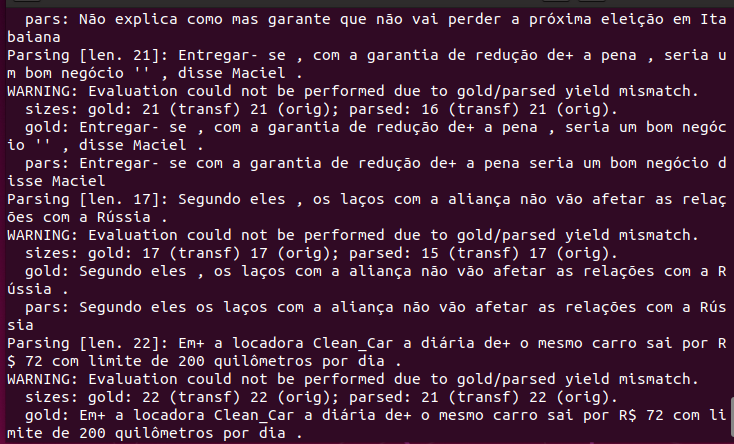
\includegraphics[width=.8\textwidth,scale=1.5]{imagens/erro_mismatch.png}
    \caption[Erro de não casamento (\textit{mismatch}) entre árvores]{Erro de não casamento (\textit{mismatch}) entre árvores ao executar o SP sobre o Bosque pré-treinado.}
    \label{fig:bosque_erro_mismatch}
\end{figure}
\end{center}
% ------------------------------------------------------------------------------------------------
\subsection{Problemas com CU (Coordenação)}
\label{subsec:cu}
Coordenação é uma das \textit{tags} mais problemáticas do BOSQUE. Como destacam \citeonline[p~4]{Wing2006Adaptation}:
\begin{quote}
    \textquote{\textit{Conjoined clauses in the native Floresta are of type CU, regardless of the type of constituents being conjoined. This causes grammars learned from the treebank to make errors such as conflating noun phrase conjunctions and sentential conjunctions}}.
    \footnote{\textquote{Cláusulas conjuntivas no Floresta nativo são do tipo CU, independentemente do tipo de constituinte conjunto. Isso faz com que a gramática aprendida do treebank cometa erros como confundir conjunções de sintagmas nominais e conjunções sentenciais}. Tradução própria.}.
\end{quote}

O PTB tem suas próprias regras para determinar a estrutura de coordenações, reservando o Capítulo 7 de seu \textit{Bracketing Guidelines}\footnote{Manual de Agrupamento} \cite[p~117]{bracketing_ptb}. Seguindo tais regras, num primeiro momento de tradução, apenas marcamos as coordenações com a \textit{tag} auxiliar \_CU\_. Depois, fizemos uma nova verificação, reconhecendo as sentenças onde essa marca aparece.
\begin{center}
    \begin{figure}[!h]
    \centering
    \begin{minipage}{10cm}
        \begin{tabbing}
            \=(\textbf{H:cu}\=\+ \\
            \>    (CJT:\=np \+\\
            \>        (H:n:saúde:F\_S::anr\_np-def: saúde))\-\\
            \>    \=(CO:conj-c:e:::: e)\\
            \>    (CJT:\=np \+\\
            \>        (H:n:educação:F\_S::np-idf: educação)))))))
        \end{tabbing}
    \end{minipage}
    % \includegraphics{}
    \caption[Exemplo de uso do sintagma evidenciador de coordenação no Bosque]{Exemplo de uso do sintagma evidenciador de coordenação no Bosque. Fragmento da sentença CF5-2}
    \label{fig:bosque_exemplo_cu}
\end{figure}
\end{center}

Já citamos, em \ref{subsec-cintil-conj}, que o PTB lida com a coordenação de basicamente três formas: palavras simples, palavras múltiplas e conjunções descontínuas. A \textit{tag} \textit{cu} define o sintagma que encabeça a coordenação. Isto pode ser melhor visto na Figura \ref{fig:bosque_exemplo_cu}. Isto facilita o procedimento pois, deve-se então verificar se os sintagmas filhos possuem a mesma \textit{tag}, e se são nós terminais ou não-terminais. Sendo terminais, devem ser impressos numa estrutura achatada (\textit{flat structure}). Sendo não-terminais, de mesma categoria, a \textit{tag} cu deve ser convertida para uma \textit{tag} equivalente. Sendo sintagmas de categorias distintas, cu é convertido para UCP (\textit{Unlike Coordinated Phrase}\footnote{\textquote{Sintagma Coordenado Diferente}. Tradução própria.}).
\begin{center}
    \begin{figure}[!h]
    \centering
    \begin{minipage}{10cm}
        CF766-6 E o Brasil?
        \begin{tabbing}
            \=(FRASE\=  CF766-6 (QUE:np (\textbf{CO:conj-c:e:: E})\+\\
            \>    (>N:art:o:M\_S::artd: o)\\
            \>    (H:prop:Brasil:M\_S::: Brasil)\\
            \>    (?)))\\
        \end{tabbing}
    \end{minipage}
    % \includegraphics{}
    \caption[Exemplo árvore onde palavra marcada por conj-c não implica em conjunção entre sentenças]{Exemplo árvore onde palavra marcada por conj-c (conjunção coordenativa) não implica em conjunção entre sentenças}
    \label{fig:bosque_exemplo_conj-c}
\end{figure}
\end{center}

Tem-se, também, que tomar cuidado com os casos de palavras simples, em \textit{flat structure}. Por dois motivos: primeiro, não necessariamente uma palavra que, no Bosque, é marcada por conj-c (conjunção coordenativa), será um indicador de conjunção, efetivamente. Exemplo na sentença CF766-6, Figura \ref{fig:bosque_exemplo_conj-c}. Nesses casos, a palavra deve ser marcada com a \textit{tag} CC para o PTB. O segundo problema é a correta escrita da \textit{flat structure}. O \cite[p~117]{bracketing_ptb}  mostra alguns exemplos possíveis. Empiricamente, notamos que a forma correta deve ser como na Figura \ref{fig:bosque_exemplo_flat}, ou seja, o valor pós-conjunção deve ser destacado num novo sintagma.
\begin{center}
    \begin{figure}[!h]
    \centering
    \begin{minipage}{10cm}
        \begin{tabbing}
            \=(VP \=\+\\
            \>    (IN \=porque)\+\\
            \>        (VP \=\+\\
            \>            (VBP tem)\-\\
            \>        )\\
            \>        (NP \=\+\\
            \>            (NN gente)\-\\
            \>        )\\
            \>        (VP \=\textbf{comprando e}\+\\
            \>            (\textbf{VBG vendendo})))
        \end{tabbing}
    \end{minipage}
    % \includegraphics{}
    \caption[Exemplo de como coordenações \textit{single word} devem se comportar]{Exemplo de como coordenações \textit{single word} devem se comportar. Fragmento da conversão da sentença \textit{CF400-2 Diretor do Banco Central não acredita que o real esteja valorizado porque \guillemotleft tem gente comprando e vendendo\guillemotright}}
    \label{fig:bosque_exemplo_flat}
\end{figure}


\end{center}
% ------------------------------------------------------------------------------------------------
\subsection{O par \textbf{x} e \textbf{X}}
\label{subsec:sec_x}
Ainda há, no \textit{corpus}, o par de \textit{tags}, X e x. X é uma \textit{tag} do tipo função, e x uma \textit{POS tag}. Na Bíblia Florestal (\cite{freitas2007biblia}), não há uma descrição formal para ambas. Apenas notou-se que nunca aparecem em par, mas quase sempre próximas. Num primeiro momento, a solução foi ignorar este par, descartando toda sentença / árvore em que aparecem. Mas uma revisão mostrou que seria uma grande perda desprezá-los, e isso nos levou a uma série de desdobramentos interessantes.
\begin{center}
    \begin{table}[!h]
    \centering
    \begin{tabular}{|l|r|l|r|}
    \hline
        X:adv   &   1   &   CJT:x   &   480\\
        X:cu    &   22  &   EXC:x   &   1\\
        X:np    &   3   &   N<:x    &   18\\
        X:pp    &   130 &   P<:x    &   1\\
        	    &       &   PIV:x   &   3\\
        	    &	    &   UTT:x   &   2\\
        \hline
    \end{tabular}
    \caption{Pares possíveis para as tags X, e frequência de aparecimento no CETEMFolha}
    \label{tab:tag_X}
\end{table}
\end{center}

Na Tabela \ref{tab:tag_X}, mostramos quais as ocorrências das \textit{tags} X e x, em conjunto com seus possíveis pares (ou seja, \textquote{$(F:x)$ e $(X:f)$}, sendo \textit{f} e \textit{F} \textit{tags} quaisquer). Pode-se notar que, por mais que ambas sejam casadas com diversas etiquetas, no geral se associam à \textit{tags} de conjunção. Uma hipótese, então, é:
\begin{quote}
	X e x são \textit{tags} coringas. Elas ocupam o espaço da Função ou da Forma (respectivamente) quando a informação realmente relevante é apenas o seu par. 
\end{quote}

Isto gera um problema. Como descrito em \ref{subsec:florestasintatica}, todo nó tem pelo menos o par F:f, e como foi dito no começo da seção, deu-se preferência às \textit{tags} \textit{forma} (por serem equivalentes às \textit{POS tags}) em detrimento às outras. As \textit{tags} x nos forçam a voltar a olhar para as \textit{tags} irmãs. Ou seja, nos casos em que o nó possui uma \textit{tag} x, F informará o valor a ser convertido. As \textit{tags} F, então, necessitam de uma nova tabela, que pode ser vista na Tabela \ref{tab:bosque_func_edit}.
\begin{center}
    \begin{longtable}{|p{0.1\linewidth}|p{0.2\linewidth}|p{0.15\linewidth}|p{0.15\linewidth}|p{0.3\linewidth}|}
\caption{Tabela de conversão: BOSQUE para PTB (Funções relevantes)}\\
\hline
\textbf{Tag Original (Português)} & \textbf{Nome da Tag} & \textbf{Tag Convertida} & \textbf{Ocorrências} & \textbf{Observações}\\
\hline
\endfirsthead
\multicolumn{5}{c}%
{\tablename\ \thetable\ -- \textit{Continuação da página anterior}} \\
\hline
\textbf{Tag Original (Português)} & \textbf{Nome da Tag} & \textbf{Tag Convertida} & \textbf{Ocorrências} & \textbf{Observações} \\
\hline
\endhead
\hline \multicolumn{5}{r}{\textit{Continua na próxima página}} \\
\endfoot
\hline
\endlastfoot
    \textgreater A & dependente em adjp ou advp (antecede o núcleo) & \textgreater A & 371 & Explicado em \ref{subsec:bosque_a} \\
    A\textless & dependente em adjp ou advp (segue o núcleo) & A\textless & 272 & Explicado em \ref{subsec:bosque_a} \\
    ACC & objecto directo (incluindo alguns tipos de se) & depende da \textit{form\_tag} & 4315 & Explicado em \ref{subsec:tag_acl}\\
    ADVL & adjunto adverbial & depende da form & 6032 & Explicado em \ref{subsec:tag_acl}\\
    CJT & elemento conjunto & \_CJT\_ & 3945 & Explicado em \ref{subsec:CJT}\\
    EXC & enunciado exclamativo & S & 36 & \\
    H & núcleo & depende da form & 40148 & \\
    KOMP\textless  & complemento comparativo & \_KOMP\_ & 40 & Explicado em \ref{subsec:tag_komp}\\
    \textgreater N & adjunto adnominal (antecede o núcleo) & NP & 14009 & Dobra do NP por adjunto, como visto em \citeonline[p~67]{mioto2013novo}
    \footnote{\citeonline[p~67]{mioto2013novo} descreve a dobra de sintagmas para adjuntos.
    \begin{quote}
        \textquote{[\ldots] existem ainda sintagmas que são licensiados numa sentençça sem serem complemento ou especificador de um núcleo. São os chamados \textbf{adjuntos}. [\ldots] Um adjunto [\ldots] é um sintagma que está apenas contido na projeção máxima de um núcleo. [\ldots] A representação do adjunto sempre implica a duplicação da categoria com a qual ele está relacionado. Desta forma, o adjunto vai ser dominado apenas pelo segmento de cima da categoria duplicada.}
    \end{quote}}
    \\
    N< & adjunto adnominal (segue o núcleo) & NP & 9208 & Dobra do NP por adjunto, como visto em \citeonline[p~67]{mioto2013novo}\\
    OC & predicativo do objeto & depende da form & 102 & Explicado em \ref{subsec:tag_acl}\\
    \textgreater P & dependente da preposição & PP & 71 & Por observação, e por \citeonline[p~67]{mioto2013novo}\\
    P & predicador & VP & 8053 & Pela \citeonline[p~60]{afonso2006arvores}, O predicador é sempre de natureza verbal e, por isso, pode exibir apenas formas verbais\\
    P< & argumento de preposição & PP & 11574 & Por observação, e por \citeonline[p~67]{mioto2013novo}\\
    PIV & objecto preposicional & PP & 1097 & \\
    QUE & enunciado interrogativo & S & 64 & \\
    SC & predicativo do sujeito & VP & 1254 & \\
    STA & enunciado declarativo & S & 3683 & \\
    UTT & enunciado & S & 468 &

\label{tab:bosque_func_edit}

\end{longtable}
\end{center}

A Tabela \ref{tab:bosque_func_edit} é um fragmento da Tabela \ref{tab:bosque_func_full}, que pode ser encontrada nos apêndices. Esta última possui, efetivamente, todas as \textit{tags} de função, seus nomes, possíveis conversões etc. Diversas delas não serão utilizadas neste trabalho, portanto não necessitam ser abordadas nesta seção.

Isso nos leva a novas questões. Nem todas as \textit{tags} de função são explícitas quanto ao sintagma que elas definem. Ou seja, uma informação de sintagma precisa seria obtida pela \textit{tag} $f$, que no caso é $x$, que não tem valor sintagmático, e o PTB não prevê sintagmas não marcados, ou etiquetas coringa. Vamos verificar essas funções nas próximas sessões, e as estratégias utilizadas para resolver tais problemas.

% ------------------------------------------------------------------------------------------------
\subsection{PROBLEMAS COM >A e A<}
\label{subsec:bosque_a}

Vemos em \cite[p~13]{afonso2006arvores}
% \begin{quote}
    \textquote{A indicação de \textquote{>} e \textquote{<} presentes nas funções acima, reflectem a posição do dependente face ao núcleo, como setas direccionadas para o núcleo cuja natureza está indicada por letras maiúsculas}. 
% \end{quote}
Vemos também que 
% \begin{quote}
    \textquote{Por outro lado, >A significa que o dependente aponta para o núcleo de natureza adjectival ou adverbial (\textquote{A}) que se encontra à direita do dependente (\textquote{>})}.
% \end{quote}

A possível ambiguidade da sentença anterior é resolvida em \cite[p~58]{afonso2006arvores}, no qual se lê \textquote{As mesmas etiquetas, A< e >A, como se pode constatar, estão presentes tanto nos sintagmas adjectivais como nos sintagmas adverbiais enquanto modificadoras de adjectivos ou advérbios}. Ou seja, para a correta conversão de >A (por exemplo) para ADVP, ou ADJP, é necessário olhar o nó irmão, e verificar o seu núcleo. Este sendo adjetivo ou sintagma adjetival, >A se torna ADVP, e análogo para advérbios. Mas o que fazer em casos como da sentença CF761-3 (Figura \ref{fig:bosque_a_seta_errado}), em que o nó irmão de >A é um advérbio, mas o núcleo do sintagma é adjetivo? 
\begin{center}
    \begin{figure}[!h]
    \centering
    \begin{minipage}{10cm}
        \ldots
        \begin{tabbing}
            \=(SC:\=adjp \+\\
            \>    (\textbf{>A}:\=x (X:pp\+\\ 
            \>          (H:prp:de:::: de)\\
            \>          (P<:\=np \+\\
            \>            (>N:num:30:M\_P::card: 30)\\
            \>            (H:n:\%:M\_P::anr\_np-count:anr\_np-def: \%)))\-\\
            \>        (X:\=pp \+\\
            \>          (H:prp:a:::: a)\\
            \>          (P<:\=np \+\\
            \>            (>N:num:40:M\_P::card: 40)\\
            \>            (H:n:\%:M\_P::anr\_np-count:anr\_np-def: \%))))\-\-\-\\
            \>    (\textbf{>A:adv}:mais:\_::KOMP:quant: mais)\\
            \>    (\textbf{H:adj}:rápido:F\_P::: rápidas)\\
            \>    (KOMP<:acl \\
        \end{tabbing}
        \ldots
    \end{minipage}
    % \includegraphics{}
    \caption[Exemplo de estrutura ambígua de >A]{Exemplo de estrutura ambígua de >A. Fragmento da árvore da sentença CF761-3 \textquote{As novas impressoras a laser da HP vêm com um novo padrão de velocidade 12 páginas por minuto (ppm) e são de 30\% a 40\% mais rápidas que as da geração anterior}.}
    \label{fig:bosque_a_seta_errado}
\end{figure}

\end{center}

Para este trabalho, os nós não conservam as informações de função, apenas de forma. Assim sendo, >A será transduzido de acordo com o primeiro nó válido na direção indicada por > ou <.
% ------------------------------------------------------------------------------------------------
\subsection{PROBLEMAS COM CJT (Conjunção)}
\label{subsec:CJT}
Ainda sobre sintagmas evidenciadores da relação de coordenação (visto em \ref{subsec:cu}), \cite[p~20]{afonso2006arvores} descreve: 
\begin{quote}
    \textquote{A sua estrutura interna evidencia também a relação de coordenação: duas ou mais partes coordenadas como função e uma ou mais conjunções coordenativas, que podem ou não estar presentes. A forma de cada uma das partes coordenadas segue os princípios gerais dos sintagmas não verbais, isto é, dependendo da sua estrutura interna e em particular da função dos dependentes do núcleo do sintagma, ou dos sintagmas verbais}.
\end{quote}

As \textquote{partes coordenadas} citadas são nós cuja função é CJT. Como é melhor explorado em \cite[p~96]{afonso2006arvores} \textquote{nós dependentes daquele, terminais ou não terminais, ao mesmo nível que correspondem às partes coordenadas $(CJT: forma)$}.

Quando tal tipo de função ocorre para um nó, a solução de transdução costuma ser simples: basta utilizar o valor de forma. O problema, claro, é que estamos aqui justamente por nossa \textit{forma} ser \textquote{x}, a etiqueta \textquote{coringa}. Nestes casos, empiricamente, notou-se uma frequência alta de sentenças internas à $(CJT:x)$ que possuem valor sintático de sintagma verbal (VP). Portanto, decidimos que os casos $(CJT:x)$ seriam convertidos para VP.
\begin{center}
    \begin{table}[!h]
    \centering
    \begin{tabular}{|l|r|l|r|}
        \hline
        CJT\&ACC:np & 1 & CJT:fcl & 596\\
        CJT\&ADVL:pp & 3 & CJT:icl & 123\\
        CJT\&PASS:pp & 1 & CJT:n-adj & 12\\
        CJT\&PRED:adjp & 2 & CJT:np & 1990\\
        CJT:acl & 12 & CJT:pp & 392\\
        CJT:adjp & 288 & CJT:v-ger & 2\\
        CJT:advp & 24 & CJT:v-pcp & 22\\
        CJT:cu & 6 & CJT:x & 480\\
        \hline
    \end{tabular}
    \caption{Possíveis combinações de CJT.}
    \label{tab:bosque_CJT}
\end{table}
\end{center}

Podemos ver na Tabela \ref{tab:bosque_CJT} a frequência com quem CJT se pareia, e vemos nele uma certa \textit{tag} chamada acl. Na Tabela \ref{tab:tab_bosque} podemos ver que ela merece uma atenção especial. Dedicaremos um pouco mais de tempo à ela.
% ------------------------------------------------------------------------------------------------
\subsection{PROBLEMAS COM ACL (ORAÇÕES AVERBAIS)}
\label{subsec:tag_acl}
Vemos em \cite{freitas2007biblia}, \textquote{Finalmente, na oração averbal
\footnote{Note que, em \cite[p~12]{afonso2006arvores}, acl é grifada como \textquote{oração deverbal}}
\footnote{\textquote{the crawling chaos\ldots}. \citeonline{lovecraft1920nyarlathotep}}
, o verbo não está presente, mas normalmente estas orações são encabeçadas por uma conjunção subordinativa que indica a natureza oracional do período}. Ao passo que fcl e icl (orações finitas e não-finitas) podemos afirmar serem conversíveis para VP, acl nos obriga a fazer conversões para a forma de oração subordinada \cite[p~172]{bracketing_ptb}, porém também não de forma assertiva. Pois, como vemos na Tabela \ref{tab:bosque_acl}, acl pode se ligar a qualquer forma sintagmática, inclusive início de orações. Porém, observar a função costuma dar uma informação bastante definitiva, conversão que adotamos nos casos de ADVL:acl, EXC:acl, N<:acl, N<PRED:acl, QUE:acl, STA:acl, UTT:acl. Para casos como ACC:acl e OC:acl, tomamos opções arbitrárias: convertemos para NP. Faltam dois casos então, KOMP< e CJT (novamente).
\begin{center}
    \begin{table}[!ht]
    \centering
    \begin{tabular}{|l|r|l|r|}
        \hline
        ACC:acl     &   1   &   N<PRED:acl  &   6\\
        ADVL:acl    &   78  &   OC:acl  &   31\\
        CJT:acl     &   12  &   QUE:acl &   1\\
        EXC:acl     &   4   &  	SC:acl  &   15\\
        KOMP<:acl   &   44  &   STA:acl &   3\\
        N<:acl      &   40  &   UTT:acl &   63\\
        \hline
    \end{tabular}
    \caption{Possíveis combinações da \textit{tag} \textit{acl}, e frequência de ocorrência no CETEMFolha}
    \label{tab:bosque_acl}
\end{table}
\end{center}
% ------------------------------------------------------------------------------------------------
\subsection{PROBLEMAS COM KOMP< (COMPLEMENTOS)}
\label{subsec:tag_komp}
Esta etiqueta é definida, por \cite[p~57]{afonso2006arvores} como \textquote{KOMP<, segundo termo de uma oração comparativa ou oração consecutiva}. E em \cite[p~116]{afonso2006arvores}:
\begin{quote}
    \textquote{Em termos de representação em árvores, a particularidade é o segundo termo de comparação ser etiquetado com KOMP< (etiqueta de sintagma) ao mesmo nível de constituintes que o adjectivo ou advérbio e o seu dependente. [\ldots] KOMP< terá como forma \textquote{fcl}, no caso de o verbo principal estar expresso ou \textquote{acl}, no caso de o verbo principal estar omisso}.
\end{quote}

É reservado o Capítulo 22 do \cite[p~284]{bracketing_ptb} para o estudo de comparativos. Nele, vemos:
\begin{quote}
    \textquote{\textit{The than, that, or as is bracketed as either a PP or an SBAR, and a certain amount of variations exists in the choice of PP, or SBAR. SBAR is used when the rest of the than/that/as-phrase is a tensed sentence, or when it contains a subject. PP is in general when the rest of the than/that/as-phrase is a single constituent [\ldots]}}.
\end{quote}

Dois exemplos simples podem ser vistos na Figura \ref{fig:ptb_exemplo_comp}. Foi necessário, então, repetir tal comportamento na transdução.
\begin{center}
    \begin{figure}[!h]
    \centering
    \begin{minipage}{.3\linewidth}
        \ldots
        \begin{tabbing}
            \=(PP \=than/as\+\\
            \>    (xP rest of phrase))\\
            \>\\
        \end{tabbing}
        \begin{tabbing}
            \=(SBAR \=than/that/as\+\\
            \>    (S rest of phrase))\\
        \end{tabbing}
        \ldots
    \end{minipage}
    % \includegraphics{}
    \caption[Exemplos de configurações das sentenças comparativas no PTB]{Exemplos de configurações das sentenças comparativas no PTB. Adaptado de \cite[p~284]{bracketing_ptb}}
    \label{fig:ptb_exemplo_comp}
\end{figure}




\end{center}
% ------------------------------------------------------------------------------------------------
\subsection{PROBLEMAS COM CJT:acl}
\label{subsec:CJT_acl}
Definitivamente, a mais desafiadora das conversões. Sentenças averbais com valor de conjunção. Não existe uma forma precisa de converter este par. 

Notou-se também que observar os nós filhos, ou mesmo os pais, não nos dariam informações precisas que nos permitisse afirmar qual seria uma transdução interessante, que fosse reconhecível tanto por PTB como por SP. Ser arbitrário, e defini-lo como VP ou NP, por exemplo, causaria muitos problemas. Não restava muitas escolhas. Como trabalho futuro, caberá o estudo deste par. Por ora, decidiu-se transduzí-los para \textquote{S} (marcador de Sentença).
% ------------------------------------------------------------------------------------------------
\subsection{PROBLEMAS COM O BOSQUE}
\label{subsec:erros_bosque}
Dentre as dificuldades na transdução Bosque/PTB, alguns erros no \textit{dataset} merecem ser frisados. Como já dito, o Bosque originalmente é distribuído no formato Árvores Deitadas, mas possui uma distribuição em formato \textit{Penn Treebank}. A observação nos mostra que, na prática, apenas foram substituídos os símbolos de indentação pelos parênteses do PTB. 
% Nos apêndices, haverá uma lista completa os que foram detectados por nós. 
% Neste momento, serão destacados alguns casos.
Destacam-se alguns casos.

P.vp - Na sentença CF624-3, a separação de etiquetas está incorreta. Ao invés de estar escrito \textquote{P:vp}, está grifado \textquote{P.vp}, como visto na Figura \ref{fig:bosque_erro_pvp}.

\begin{center}
    \begin{figure}[!h]
    \centering
    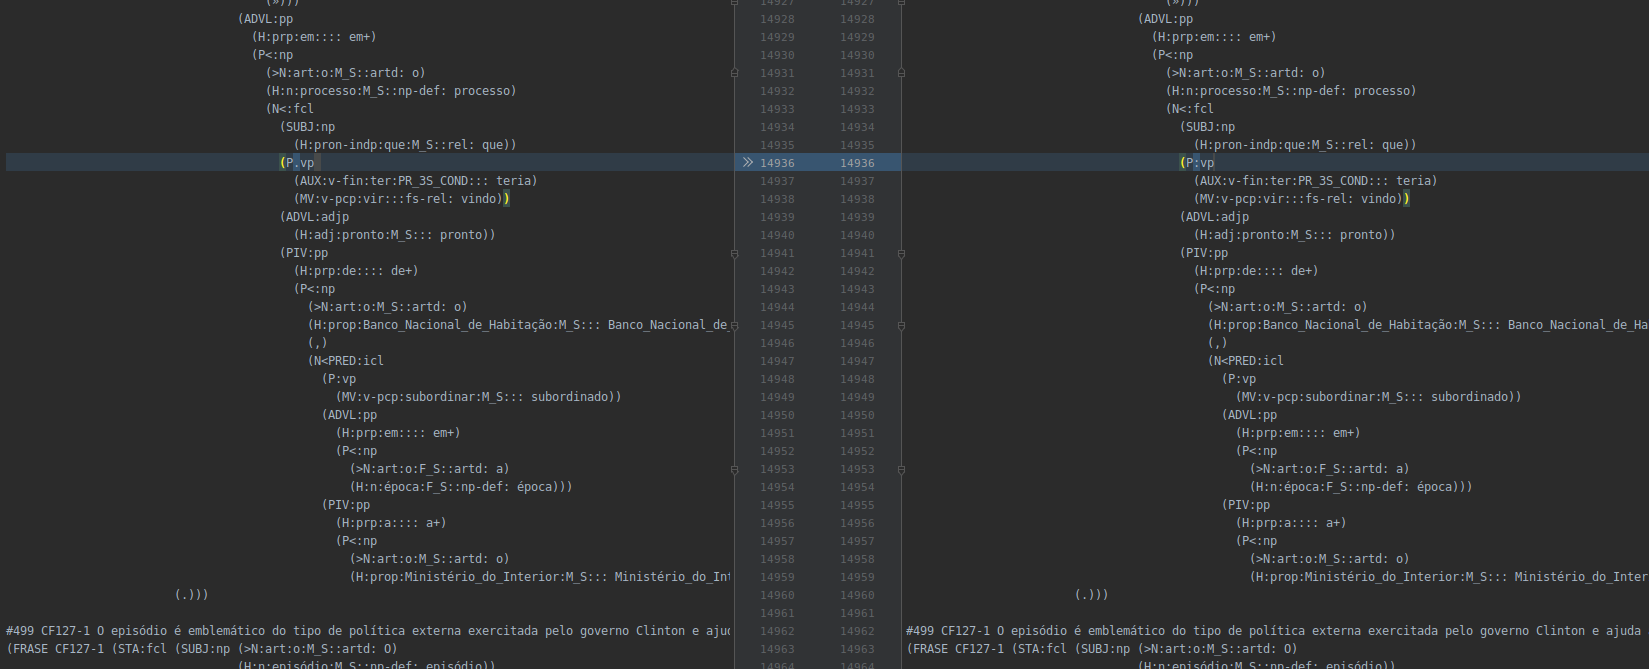
\includegraphics[width=\textwidth,scale=1.5]{imagens/erro_escrita_498.png}
    \caption[Erro na marcação do par P:vp]{Erro na marcação do par P:vp}
    \label{fig:bosque_erro_pvp}
\end{figure}
\end{center}

Nó terminal fechado de forma incorreta - Alguns nós que necessariamente são terminais (como determinantes, ou pronomes) ocorrem fechados de forma inconsistente. A correção foi necessária. A sentença CF624-3 contém um exemplo, que pode ser visto na Figura \ref{fig:bosque_erro_no_fechado_errado}.

\begin{center}
    \begin{figure}[!h]
    \centering
    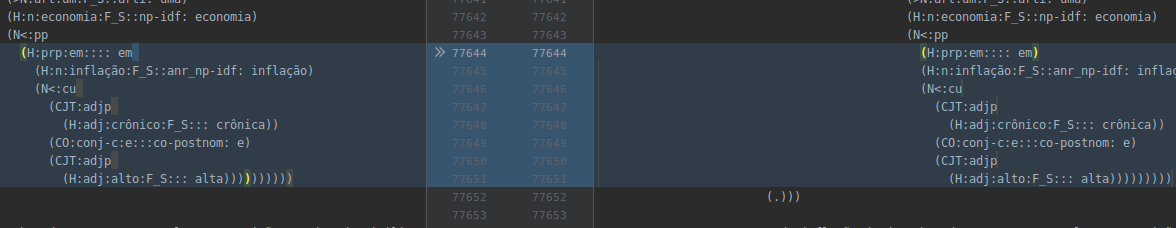
\includegraphics[width=\textwidth,scale=1.5]{imagens/erro_escrita_2626.png}
    \caption[Erro no fecho do nó H:prp]{Erro no fecho do nó H:prp}
    \label{fig:bosque_erro_no_fechado_errado}
\end{figure}
\end{center}

Símbolos marcados incorretamente - Bosque apresenta símbolos entre parentes, sem etiquetas. Isto ocorre em duas sentenças. Um exemplo é na sentença CF322-3, como pode ser visto na Figura \ref{fig:bosque_erro_simbolos}, com o parênteses abrindo para o símbolo, mas sem o fecho na sequência. 

\begin{center}
    \begin{figure}[!h]
    \centering
    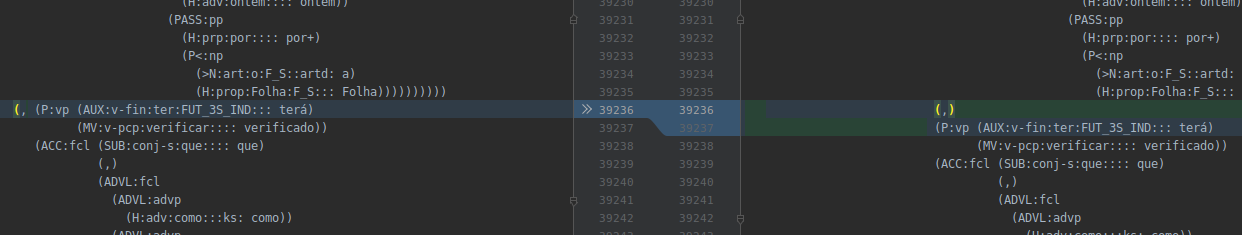
\includegraphics[width=\textwidth,scale=1.5]{imagens/erro_escrita_1340.png}
    \caption[Erro na marcação de símbolos]{Erro na marcação de símbolos}
    \label{fig:bosque_erro_simbolos}
\end{figure}
\end{center}

% ------------------------------------------------------------------------------------------------
\subsection{Treinamento}
\label{subsec:treinamento_bosque}
De modo análogo ao CINTIL, fizemos o treinamento baseado num comando simples, como visto no código \ref{lst:treinoBasicoBosque}
\begin{center}
    \begin{lstlisting}[breaklines, caption={Execução de treinos do Stanford Parser para o Bosque},label={lst:treinoBasicoBosque},language=Bash]
    java -cp stanford-parser.jar -mx4g edu.stanford.nlp.parser.lexparser.LexicalizedParser -train ~/<diretorio do treebank> 1-421 -saveToSerializedFile ~/<diretorio de armazenamento>/serialGrammarBOSQUE1 > ~<diretorio de armazenamento>/outputs/treinoBOSQUE/treinoBr1.txt
\end{lstlisting}

\end{center}

São comandos análogos aos utilizados para CINTIL. Explicações podem ser vistas na Tabela \ref{tab:tab_treino_basico_cintil}.

Para a execução dos testes, foi utilizado o comando \ref{lst:testeBasicoBosque}
\begin{center}
    \begin{lstlisting}[breaklines, caption={Execução de testes do Stanford Parser para o Bosque},label={lst:testeBasicoBosque},language=Bash]
    java -cp stanford-parser.jar -mx4g edu.stanford.nlp.parser.lexparser.LexicalizedParser -writeOutputFiles -outputFilesDirectory ~/<diretorio de relatorios de treino>/treino -loadFromSerializedFile ~/<diretorio da gramatica serializada>/serialGrammarBOSQUE1 -testTreebank ~/<diretorio dos treebanks> 422-4213 > ~/<diretorio dos resultados dos testes>testeBr1.txt
\end{lstlisting}

\end{center}

É o mesmo comando explicado na Tabela \ref{tab:tab_teste_basico_cintil}. Também foi utilizado o \textit{10-fold validation} para o Bosque. Porém, os testes foram feitos majoritariamente com o CETEMFolha, que possui 4213 sentenças (contra 10140 do CINTIL).

O resultado completo dos testes pode ser visto na Tabela \ref{tab:bosque_result_full}, nos apêndices. Os comentários dos resultados pode ser visto em \ref{resultados_bosque}.
